\section{Background and Related Works}
\label{sec:background}
%UPPRESSO is designed to be compatible with OpenID Connect (OIDC) and provide privacy protections based on the discrete logarithm problem. Next,

This section introduces the popular OIDC \cite{OpenIDConnect},
 to explain typical SSO login flows.
Then, we discuss existing privacy-preserving SSO solutions and other related works.

\subsection{OpenID Connect}
\label{subsec:OIDC}
OIDC is one of the most popular SSO protocols \cite{OpenIDConnect} for web applications. %As other SSO protocols \cite{SAMLIdentifier}, OIDC
%It involves three entities, i.e., {\em users}, the {\em identity provider (IdP)}, and {\em relying parties (RPs)}.
Users and RPs register at the IdP with their identities %($ID_U$, $ID_{RP}$ and $PID_U$ in some schemes) %(or $PID_{RP}$ in some schemes)
and other necessary information such as user credentials (i.e., passwords or public keys)
 and RP endpoints (i.e., the URLs to receive identity tokens).
% below can be removed
%The IdP should maintain these attributes securely.

\vspace{1mm}
\noindent\textbf{Implicit Login Flow.}
OIDC supports three types of user login flows: implicit flow, authorization code flow, and hybrid flow (i.e., a mix-up of the previous two).
%In the implicit flow, an {\em id token} is generated as the identity token, which contains a user identifier, an RP identifier, the issuer (i.e., IdP), the validity period, and other requested attributes. The IdP signs the id token using its private key to ensure integrity, and sends it to the RP through the user.
%In the authorization code flow, the IdP binds an authorization code with the RP, and sends it to the RP through the user; then, the RP establishes an HTTPS connection to the IdP and uses the authorization code with the RP's credential to obtain the user's identifier and other attributes.
%UPPRESSO is compatible with all three flows.
These flows mainly result from the differences of the communication steps to request and receive identity tokens,
    but work with the common security requirements of identity tokens.
We introduce the implicit flow and present our design and implementation based on this flow,
    the extensions to support the authorization code flow will be discussed in Section \ref{sec:discussion}.

\begin{figure}[t]
  \centering
  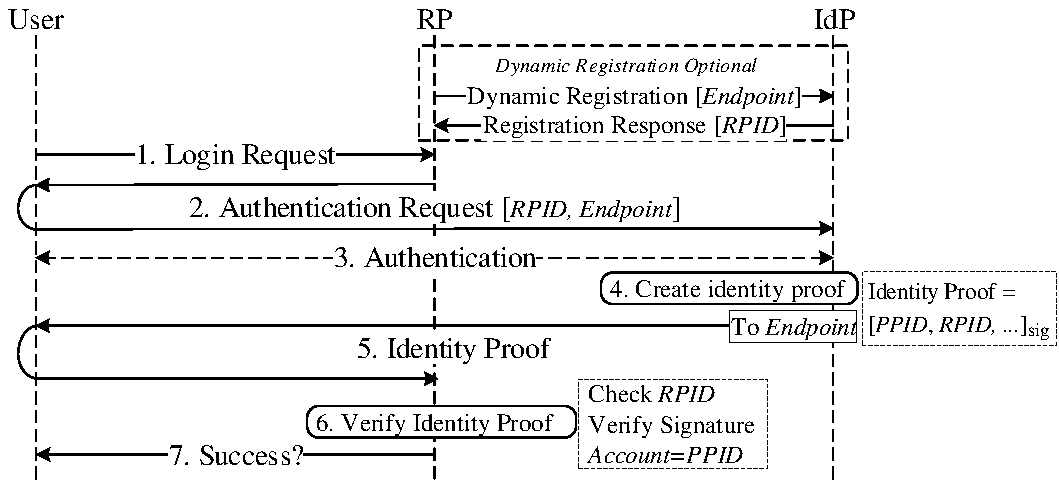
\includegraphics[width=0.9\linewidth]{fig/OIDC1.pdf}
  \caption{The implicit SSO login flow of OIDC.}
  \label{fig:OpenID}
%  \vspace{-5mm}
\end{figure}

As shown in Figure \ref{fig:OpenID}, a user firstly initiates a login request to an RP.
Then, the RP constructs an identity-token request with its own identity,
% the endpoint to receive the identity token % endpointӦ��Ԥ��ע�ᡢ�̶���
 and the scope of requested user attributes.
This identity-token request is redirected to the IdP.
After successfully authenticating the user,
    the IdP issues an identity token
        which is forwarded by the user to the RP endpoint.
The token contains a user identity (or pseudo-identity),
    the RP identity, a validity period, the requested user attributes, etc.
%% If the RP endpoint has not been registered at the IdP, the IdP will return a warning to notify the user about potential identity token leakage. % ����ֻ��̸���ߣ����ִ������̫�࣬�ٲ�ʤ��
Finally, the RP verifies the received identity token and
 allows the user to login as the identity in this token.

Before issuing the identity token,
    the IdP obtains the user's authorization to enclose the requested user attributes.
%The identity token is usually signed by the IdP,
%    and transmitted through secure channels such as TLS/HTTPS.
The user's operations including authentication, redirection, authorization, and forwarding,
    are implemented in a software called \emph{user agent} (i.e., a browser for web applications).

%extracts user's identifier and returns the authentication result to the user (Step 7).

\vspace{1mm}
\noindent\textbf{RP Dynamic Registration.}
In addition to the out-of-band registrations,
    OIDC also supports dynamic registrations
    for an RP to register by online means \cite{DynamicRegistration}.
The (unregistered) RP sends a registration request
        with an endpoint to receive identity tokens and other optional information,
        to the IdP's dynamic-registration endpoint.
After a successful registration,
 the IdP assigns a unique $ID_{RP}$ to this RP in the response.


%UPPRESSO leverages this function and slightly modifies the dynamic registration process to implement the {\em $PID_{RP}$ registration} process (see details in Section \ref{sec:UPPRESSO}.C), which allows an RP to generate different privacy-preserving RP identifiers and register them with the IdP.

\subsection{Existing Privacy-Preserving Solutions for SSO}
\label{subsec-solutions}
Pairwise pseudonymous identifiers (PPIDs) are recommended by NIST \cite{NIST2017draft}
 and specified in several SSO protocols \cite{OpenIDConnect, SAMLIdentifier} to protect user privacy from curious RPs.
That is,
    when issuing an identity token,
        the IdP encloses a user pseudo-identity (but not the user identity at the IdP) in the token.
Given a user,
    the IdP assigns a unique PPID based on the target RP,
    so that collusive RPs cannot link the user's different PPIDs across these RPs.
However, PPID-based approaches cannot prevent the IdP-based login tracing,
 since  to generate identify tokens the IdP still needs to know which RP the user visits.

BrowserID \cite{BrowserID} and SPRESSO \cite{SPRESSO} are proposed to defend SSO services against the IdP-based login tracing,
    but both solutions are instead vulnerable to the threat of RP-based identity linkage.
In BrowserID (and its prototypes known as Mozilla Persona \cite{persona} and Firefox Accounts \cite{FirefoxAccount}),
 the IdP issues a special ``token'' to bind the user identity to a short-lived public key,
 so that the user uses the corresponding private key to sign a ``subsidiary'' identity token
    to bind his identity with the target RP's identity and send both tokens to the RP.
When a user logins different RPs, the RPs could still extract the identical user identities
    from different pairs of tokens and link these logins.
Meanwhile,
    the RP of SPRESSO creates a one-time but verifiable pseudo-identity for itself in each login instance.
Then, the IdP generates an identity token binding this RP pseudo-identity and the user identity. %and returns it through a trusted third-party entity called forwarder.
Similarly, the RPs could link a user's multiple logins based on his unique user identity in these tokens.

It is worth noting that PPIDs cannot be directly integrated in either BrowserID or SPRESSO.
PPIDs are assigned in identity tokens based on the visited RP \cite{NIST2017draft,OpenIDConnect, SAMLIdentifier},
    but the IdP receives (\emph{a}) nothing about the visited RP in BrowserID
     or (\emph{b}) an ephemeral pseudo-identity of the RP in SPRESSO.


\begin{comment}

\subsection{Discrete Logarithm Problem}
\label{sec:dlp}


Based on the discrete logarithm problem, UPPRESSO designs the identifier-transformation functions. %$\mathcal{F}_{ID_{RP} \mapsto PID_{RP}}$ and $\mathcal{F}_{ID_{U} \mapsto PID_{U}}$ to generate privacy-preserving user identifier (e.g. $PID_U$) and RP identifier (e.g. $PID_{RP}$), respectively.
Here, we briefly review the discrete logarithm problem.
%A number $g$ ($0<g<p$) is called a primitive root modular a prime $p$, if for ${\forall}y$ ($0<y<p$), there is a  number $x$ ($0\le x <p-1$) satisfying $y=g^x \pmod p$.
For the finite field $GF(p)$ where $p$ is a large prime, a number $g$ is called a generator of order $q$, if it constructs a cyclic  group of $q$ elements by calculating $y=g^x \ mod\ p$.
And $x$ is called the discrete logarithm of $y$ modulo $p$. Given a large prime $p$, a generator $g$ and a number $y$, it is computationally infeasible to solve the discrete logarithm (i.e., $x$) of $y$ \cite{WXWM}, which is called the discrete logarithm problem.
The hardness of solving discrete logarithms is utilized to design several secure cryptographic primitives, including Diffie-Hellman key exchange and the digital signature algorithm (DSA).

%In the process of $F_{PID_{RP}}$ and $F_{PID_U}$, we needs to calculate the primitive root for a  large prime $p$ as follows \cite{Shoup,Wang}. First, we retrieve a primitive root $g_m$  modulo $p$ from all the integers by finding the first integer passing  the primitive root checking.  A lemma is propose to simply the checking, that if $p=2q+1$ ($q$ is a prime),  an integer $\mu \in (1, p-1)$ is a primitive root if and only if $\mu^2\neq 1 \ mod \ p$ and $\mu^q\neq 1 \ mod \ p$. Then, based on $g_m$, we can calculate a new primitive root $g = g_{m}^{t} mod \ p$, where $t$ is an integer coprime to $p-1$.
\end{comment}
